\documentclass[a4paper]{article}
\linespread{1.5}
\usepackage{authblk}
\usepackage[round]{natbib}
\usepackage{amssymb, amsmath}
\usepackage{url, tikz}
\usepackage{hyperref}
\usepackage[sc]{mathpazo}
\usepackage[T1]{fontenc}
\usepackage{geometry}
\geometry{verbose,tmargin=2.5cm,bmargin=2.5cm,lmargin=2.5cm,rmargin=2.5cm}
\setcounter{secnumdepth}{2}
\setcounter{tocdepth}{2}
\usepackage{url}
\usepackage[utf8]{inputenc}
\usepackage{float} 
\usepackage[nottoc]{tocbibind}

\usepackage{Sweave}
\begin{document}


\bibliographystyle{abbrvnat}

\Sconcordance{concordance:GeorgianStockParser.tex:GeorgianStockParser.Rnw:%
1 18 1 1 0 1 1 1 7 4 1 1 7 62 1 1 2 1 0 2 1 11 0 1 1 12 0 1 2 2 1 1 2 1 %
0 1 1 19 0 1 2 2 1 1 2 1 0 2 1 18 0 1 1 19 0 1 2 3 1 6 0 1 5 8 1}



\renewcommand\Authfont{\fontsize{12}{14.4}\selectfont}
\renewcommand\Affilfont{\fontsize{9}{10.8}\itshape}

\title{\textbf{Parsing Georgian Stock Market Data}}
\author{Zijie Zhu\thanks{\href{mailto:Zijie.Zhu@williams.edu}{Zijie.Zhu@williams.edu}}}
\affil{\textit{Computer Science and Statistics \\ \textit{Williams College}       \\ \textit{Williamstown, Massachusetts}\\ \textit{United States, 01267}}}
\maketitle

\setkeys{Gin}{width=0.95\textwidth}

\tableofcontents

\begin{abstract}
The \texttt{GeorgianStockParser} package provides basic tools to download data of stock market in Republic of Georgia. Basic data organizing and analyzing tools are also offered.
\end{abstract}

\section{Introduction}
\label{sec:Introduction}

The stock market in Georgia is still under development. Although the number of stocks and the volume of trades are still relatively small compared with developed economics, Georgian stock market will eventually grow, and it is the right time to be interested, if not investing yet, in the market. This package aims to provide a few tools to download and analyze the Georgian stock market, and be used as a data set updater.

\section{Stock Data Downloader}
\label{sec:Downloader}

To analyze the stock data in Republic of Georgia, we first have to get the data set. However, there are no available data sets to use, and GSE does not offer a downloadable data set. Therefore, we first have to create a stock data downloader.

\subsection{Georgian Stock Exchange Website and Data}
\label{subsec:GSE}

The Georgian Stock Exchange website is still primary compared to the websites of stock exchange centers in more developed economics. On the website, there is no direct link to download the data. However, data of stock symbols and trade results are accessible after clicking into links.

\begin{figure}[H]
\centering
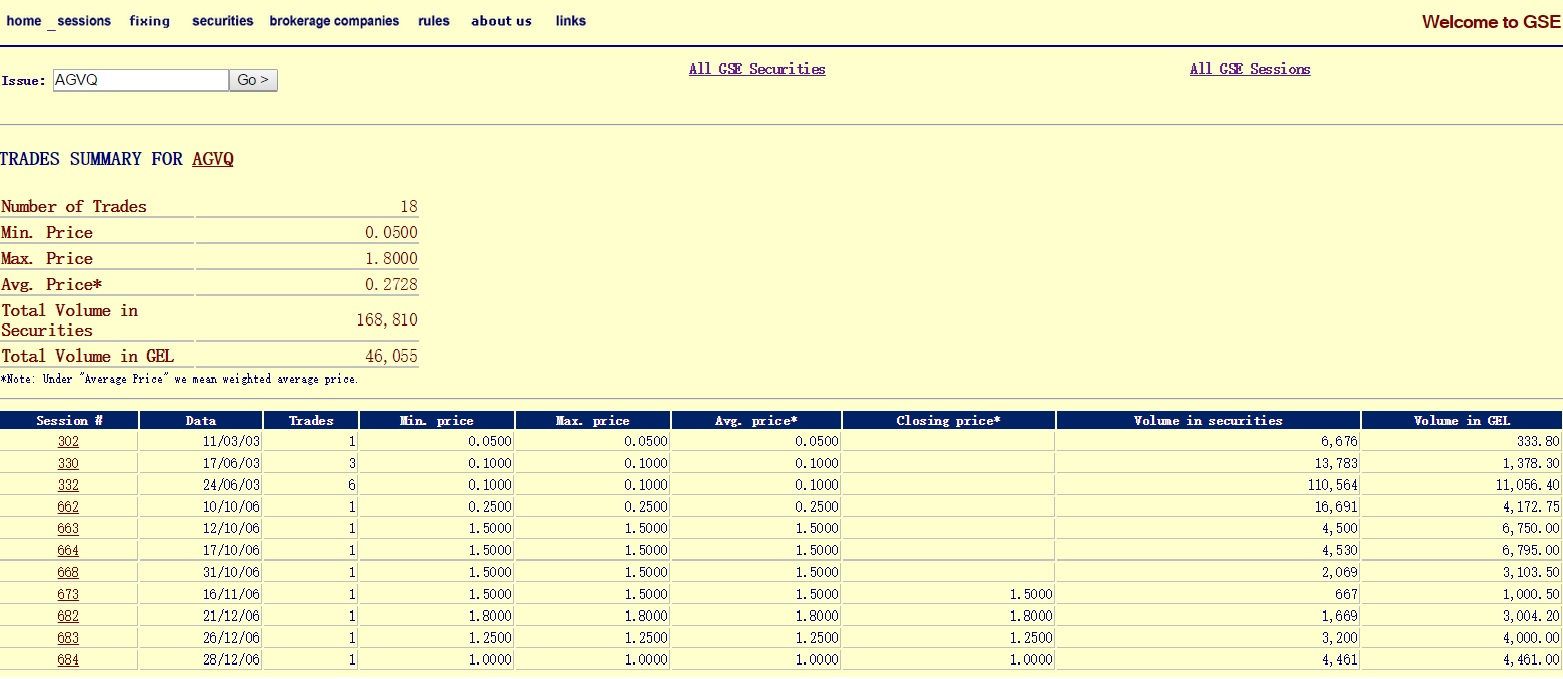
\includegraphics[width=6.3in, height=3.2in]{images/AGVQ.jpg}
\caption{GSE data taken on Jan. 14th, 2015 for Akhmeta Winery Company (stock symbol AGVQ). Information includes Session number, Date (written as ``Data'' on screenshot, probably misspelling), Trades, Min. Price, Max. Price, Avg. Price (weighted), Closing Price (weighted), Volume in Securities, and Volume in GEL (Georgian Lari). Basic summary is provided on the top-left corner. Notice that no direct download link available.}
\label{fig:AGVQ}
\end{figure}

Fortunately, the data for each stock ID are organized in an XML-accessible way. Therefore, we can use texttt{R} and \texttt{XML} package to write a downloader of the stock data.

\subsection{Downloading Functions}
\label{subsec:functions}
There are four downloading functions: \texttt{download.stockIDs}, \texttt{download.single.stock.trade}, \texttt{download.multi.stock.trade}, and \texttt{download.all.stock.trade}. 

\subsubsection{\texttt{download.stockIDs}}
\label{sssec:download.stockIDs}




\section{Conclusion}

In this paper, ...


\end{document}
